\documentclass[letterpaper,11pt,twoside]{article}
\usepackage[utf8]{inputenc}
\usepackage{amsmath,amsfonts,amssymb,amsthm,latexsym}
\usepackage[spanish,es-noshorthands]{babel}
\usepackage[T1]{fontenc}
\usepackage{lmodern}
\usepackage{graphicx,hyperref}
\usepackage{tikz,pgf}
\usepackage{marvosym}
\usepackage{multicol}
\usepackage{fancyhdr}
\usepackage[height=9.5in,width=7in]{geometry}
\usepackage{fancyhdr}
\pagestyle{fancy}
\fancyhead[LE]{\Email matematicas.german@gmail.com}
\fancyhead[RE]{\url{https://www.autistici.org/mathgerman}}
\fancyhead[RO]{\url{https://www.autistici.org/mathgerman}}
\fancyhead[LO]{\Email matematicas.german@gmail.com}

\author{Germ\'an Avenda\~no Ram\'irez~\thanks{Lic. Mat. U.D., M.Sc. U.N.}}
\title{\begin{minipage}{.2\textwidth}

\includegraphics[height=1.75cm]{Images/logo-colegio.png}\end{minipage}
\begin{minipage}{.55\textwidth}
\begin{center}
Números complejos\\
Álgebra $9^{\circ}$
\end{center}
\end{minipage}\hfill
\begin{minipage}{.2\textwidth}

\includegraphics[height=1.75cm]{Images/logo-sed.png} 
\end{minipage}}
\date{}
\thispagestyle{plain}
\begin{document}
\maketitle
Nombre: \hrulefill Curso: \underline{\hspace*{44pt}} Fecha: \underline{\hspace*{2.5cm}}
\begin{multicols}{2}
\section*{CANTIDADES IMAGINARIAS}
\subsubsection*{Actividad 1}
\begin{enumerate}
  \item Halle un número real $ x $ que cumpla:
  \begin{enumerate}\begin{multicols}{2}
    \item $ x+5=8 $
    \item $ 9-x=12 $
    \item $ x^2-9=16 $
    \item $ x^2-36=0 $
    \item $ -81+x=0 $
    \item $ x^2-4=0 $
     \end{multicols}   
  \end{enumerate}
  \item Será posible hallar un número real $ x $ tal que cumpla que:
  \[ x^2+4=0 \]
\end{enumerate}
Al intentar solucionar la anterior ecuación, llegamos al siguiente procedimiento:
\begin{align*}
  x^2+4&=0 \\
  x^2+4-4&=0-4 \qquad \text{Restando 4}\\
  x^2&=-4\\
  \sqrt{x^2}&=\pm \sqrt{-4} \qquad\text{Extrayendo raíz}\\
  x&=\pm \sqrt{-4}
\end{align*}
Como en los números reales no existe ningún valor que satisfaga la última ecuación, el proceso puede continuar de la siguiente manera:\\

$ -4 $ se puede expresar como el producto de dos cantidades, así:\\

$ -4=(4)\cdot (-1) $, luego\\
\begin{align*}
  x&=\pm \sqrt{-4} \qquad \text{se puede reemplazar por:}\\
  x&=\pm \sqrt{(4)(-1)}\\
  x&=\pm \sqrt{4}\sqrt{-1} \qquad \text{Por propiedad de la radicación}\\
  x&=\pm 2\sqrt{-1}\\
  x&=\pm 2i \qquad \text{ya que }\sqrt{-1}=i  
\end{align*}
Se ha introducido luego la unidad imaginaria \mbox{$ \sqrt{-1}=i $}. Los números que se representan de la forma $ bi $ reciben el nombre de \emph{cantidades imaginarias} y nacen de la necesidad de dar soluciones a las ecuaciones de la forma $ x^2+a=0 $\\

En la expresión $ bi $, $ b $ representa el valor de las cantidades imaginarias, mientras que $ i $ es la \emph{unidad imaginaria} cuyo valor es: $ \sqrt{-1} $
\subsection*{Operaciones con cantidades imaginarias}
\subsubsection*{Actividad 2}
Analice el siguiente ejemplo y luego realice los ejercicios propuestos\\

\textbf{EJEMPLO:} Hallar el resultado de: $ \sqrt{-16}+3\sqrt{-25}-2\sqrt{-49} $\\

\textbf{Solución:} Para tal fin escriba primero las cantidades en la forma $ bi $:

\begin{minipage}{0.45\textwidth}
  \begin{align*}
    \sqrt{-16}&=\sqrt{16(-1)}\\
    &=\sqrt{16}\sqrt{-1}\\
    &=4i
  \end{align*}
\end{minipage}
  \hfill
  \begin{minipage}{0.45\textwidth}
      \begin{align*}
    3\sqrt{-25}&=3\sqrt{25(-1)}\\
    &=3\sqrt{25}\sqrt{-1}\\
    &=3\cdot5\cdot i\\
    &=15i
  \end{align*}
  \end{minipage}
  \begin{align*}
    2\sqrt{-49}&=2\sqrt{49(-1)}\\
    &=2\sqrt{49}\sqrt{-1}\\
    &=2(7)i\\
    &=14i
  \end{align*}
  Luego reemplace y efectúe la operación así:
  \[ \sqrt{-16}+3\sqrt{-25}-2\sqrt{-49}=4i+15i-14i=5i \]
En el cuaderno resuelva:
    \begin{enumerate}
      \item $ 15\sqrt{-100}+\frac{2}{3}\sqrt{-25}-\frac{4}{7}\sqrt{-49} $
      \item $ \frac{4}{3}\sqrt{-81}-5\sqrt{-36}-\frac{9}{2}\sqrt{-16} $
      \item $ 0,7\sqrt{-25}+2,4\sqrt{-100}-0,6\sqrt{-36}+8,4\sqrt{-81} $
      \item $ \frac{2}{7}\sqrt{-100}+\frac{1}{5}\sqrt{-121}-\frac{9}{5}\sqrt{-25}+\frac{3}{7}\sqrt{-9} $
    \end{enumerate}
\subsubsection*{Actividad 3}
 \begin{enumerate}
  \item Por definición toda cantidad diferente de 0, elevada a la potencia cero ¿cuánto vale?; es decir $ a^0= $?
  \item ¿Qué sucederá si elevas $ i $ a la cero?
  \item ¿Cuánto será $ i $ elevado a la uno? Es decir, cuánto vale $ i^1= $?
  \item ¿Cuánto valdrá $ i^3 $? Descomponga $ i^3=i^2\cdot i $. Reemplace los valores.
  \item ¿Cuánto valdrá $ i^4 $?
  \item Complete la siguiente tabla
  
  \begin{tabular}{|c|p{0.5cm}|c|p{0.5cm}|c|p{0.5cm}|c|p{0.5cm}|}
  \hline $ i^0 $ & & $ i^1 $ & & $ i^2 $ & & $ i^3 $ &\\
  \hline $ i^4 $ & & $ i^5 $ & & $ i^6 $ & & $ i^7 $ &\\
  \hline $ i^8 $ & & $ i^9 $ & & $ i^{10} $ & & $ i^{11} $ &\\
  \hline $ i^{12} $ & & $ i^{13} $ & & $ i^{14} $ & & $ i^{15} $ & \\ \hline
  \end{tabular}
    \end{enumerate}
  \subsection*{Conclusiones}
  La unidad imaginaria tiene cuatro potencias básicas:
  \[ i^0=1; \qquad i^1=i;\qquad i^2=-1;\qquad i^3=-i \]
  Cualquier otro valor será la repetición de uno de los anteriores valores. Para hallar el valor basta dividir la potencia dada entre 4 y determinar el residuo para compararlo con los exponentes básicos.\\
  
  \textbf{Ejemplo:} El valor de $ i^{72} $ es 1 puesto que: 
  \begin{center}
  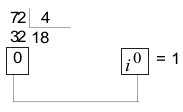
\includegraphics[scale=.5]{Images/div.png}
  \end{center}
  El valor de $ i^7 $ es $ -1 $ puesto que:
  \begin{center}
  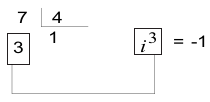
\includegraphics[scale=.5]{Images/div2.png}
  \end{center}
  \subsection*{Multiplicación y potenciación de cantidades imaginarias}
  Analizo los siguientes ejemplos y obtengo conclusiones sobre la multiplicación y potenciación de cantidades imaginarias\\
  
  \textbf{Ejemplo 1:} Desarrollar $ \sqrt{-25}\cdot 2\sqrt{-49}\cdot 3\sqrt{-\frac{25}{9}} $\\
  
  \textbf{Solución:} Se escribe cada factor en la forma $ bi $ así:\\
  
  $ \sqrt{-25}=\sqrt{25(-1)}=\sqrt{25}\cdot\sqrt{-1}=5i $\\
  
  $ 2\sqrt{-49}=2\sqrt{49(-1)}=2\sqrt{49}\sqrt{-1}=2(7)i=14i $\\
  
  $ 3\sqrt{-\frac{25}{9}}=3\sqrt{\frac{25}{9}(-1)}=3\sqrt{\frac{25}{9}}\sqrt{-1}=3(\frac{5}{3})i=5i $\\
  
  Luego \qquad $ \sqrt{-25}\cdot2\sqrt{-49}\cdot3\sqrt{-\frac{25}{9}}=5i\cdot2i\cdot5i=5\cdot2\cdot5\cdot i^3= 50(-i)=-50i $,\\
  ya que $ i^3=-i $\\
  
  \textbf{Ejemplo 2:} Efectuar $ (3i^4)^5 $\\
  
  \textbf{Solución:} Aplicando la propiedad de la potencia de un producto se tiene que:
  \begin{align*}
    (3i^4)^5&=3^5\cdot(i^4)^5\\
    &=3^5\cdot i^{20}\\
    &=3^5\cdot1 \qquad \text{(puesto que } i^{20}=1)\\
    &=243
  \end{align*}
  \subsubsection*{Ejercicios:}
  Resuelvo en mi cuaderno los siguientes ejercicios:
  \begin{enumerate}\begin{multicols}{2}
    \item $ \frac{2}{3}\sqrt{-49}\cdot\frac{1}{5}\sqrt{-36} $
    \item $ \frac{5\sqrt{-81}}{2\sqrt{9}} $
    \item $ \frac{3\sqrt{-144}}{2\sqrt{81}} $
    \item $ \dfrac{\frac{4}{3}\sqrt{-125}\cdot\frac{1}{2}\sqrt{-49}}{\frac{2}{7}}\sqrt{-49} $
    \item $ (\frac{1}{4}\sqrt{-49})^6 $
  \end{multicols} 
    \end{enumerate}
  \end{multicols}  
\end{document}
